\documentclass[12pt, oneside,a4paper]{article}
\usepackage{ctex}
\usepackage{geometry}
\usepackage{indentfirst}               		
\usepackage{listings}
\usepackage{color}
\usepackage{textcomp}
\definecolor{dkgreen}{rgb}{0,0.6,0}
\definecolor{gray}{rgb}{0.5,0.5,0.5}
\definecolor{mauve}{rgb}{0.58,0,0.82}
\usepackage{amssymb,amsmath}
\usepackage[noend]{algpseudocode}
\usepackage{algorithmicx,algorithm}
\usepackage[font=small,labelfont={bf,sf},tableposition=top]{caption}
\usepackage{graphicx}
\usepackage{multirow}
\usepackage{float}
\usepackage{fancyhdr}
\lstset{frame=tb,
  language=Python,
  aboveskip=3mm,
  belowskip=3mm,
  showstringspaces=false,
  columns=flexible,
  basicstyle={\small\ttfamily},
  numbers=none,
  numberstyle=\tiny\color{gray},
  keywordstyle=\color{blue},
  commentstyle=\color{dkgreen},
  stringstyle=\color{mauve},
  breaklines=true,
  breakatwhitespace=true,
  tabsize=3
}
\geometry{a4paper,left=2cm,right=2cm,top=3cm,bottom=3cm}

\pagestyle{fancy}
\lhead{数据库引论 Project \# 1}
\rhead{胡天晓, 张昊晗, 刘婧源}

\newcommand{\HRule}{\rule{\linewidth}{0.5mm}}
\begin{document}

\begin{titlepage}
\begin{center}
% Upper part of the page
\textsc{\LARGE 复旦大学}\\[1.5cm]
\textsc{\Large 数据库引论}\\[0.5cm]
% Title
\HRule \\[0.4cm]
{ \huge \bfseries Project 1: Glutton}\\[0.4cm]
\HRule \\[1.5cm]

\includegraphics[width=2in]{logo.jpg}\\[1cm]
% Author
\begin{minipage}{0.4\textwidth}
\begin{flushleft} \large
\begin{center}
\emph{作者:}\\
胡天晓\\
张昊晗\\
刘婧源
\end{center}
\end{flushleft}
\end{minipage}
\vfill
% Bottom of the page
{\large \today}
\end{center}
\end{titlepage}

  \makeatletter
    \renewcommand{\thefigure}{\ifnum \c@section>\z@ \thesection-\fi \@arabic\c@figure}
    \renewcommand{\thetable}{\ifnum \c@section>\z@ \thesection-\fi \@arabic\c@table}
  \makeatother

%\par\setlength{\parindent}{1em}\normalsize 
\section{项目简介}
 \begin{itemize}
  \item 项目背景
  \paragraph {Glutton数据库项目} 是为复旦大学(张江校区)的吃货们设计的外卖网页应用平台,以python链接SQL语言,web为前端,界面友好。使用者分为商家和用户,支持商家查询、创建、更改、删除菜品,用户查询商家、菜品,创建、更改、删除、评价订单等操作。
  \item 依赖库|组织架构
   flask/bootstrap/sqlite
  \item 项目文件树
  \item 运行方法
  \item flask简介
  \item bootstrap简介
  \item sqlite简介
  \item 用户密码md5加密
  \item 其他
 \end{itemize}

\section{项目细节}
 \subsection{针对用户的功能}
  \begin{itemize}
  \item 注册/登录
  \item 更改信息/头像
  \item 查找商家
  \item 下单
  \item 收货
  \item 评论
  \end{itemize}
 \subsection{针对商家的功能}
  \begin{itemize}
  \item 注册/登录
  \item 更改信息
  \item 增加菜品
  \item 删除菜品
  \item 修改菜品
  \item 查看商家订单历史
  \end{itemize}

\section{数据库简介}
 \begin{itemize}
 \item 数据源
  \par\setlength{\parindent}{1em}\normalsize 数据库Glutton所用数据来源于外卖平台”饿了么“网站,以复旦大学(张江校区)为中心,选取真实的商家信息。
 \item 数据量
  \par\setlength{\parindent}{1em}\normalsize 数据选取以蔡伦路、科苑路、华佗路的商铺为主,涵盖50个商家。每个商家菜品若干,最多为17道菜,最少为4道菜,共393道菜,平均每个商家8(7.86)道菜。整个数据库包含443条商家及菜品记录。
 \item ER图
  \begin{figure}[H]
   \centering
     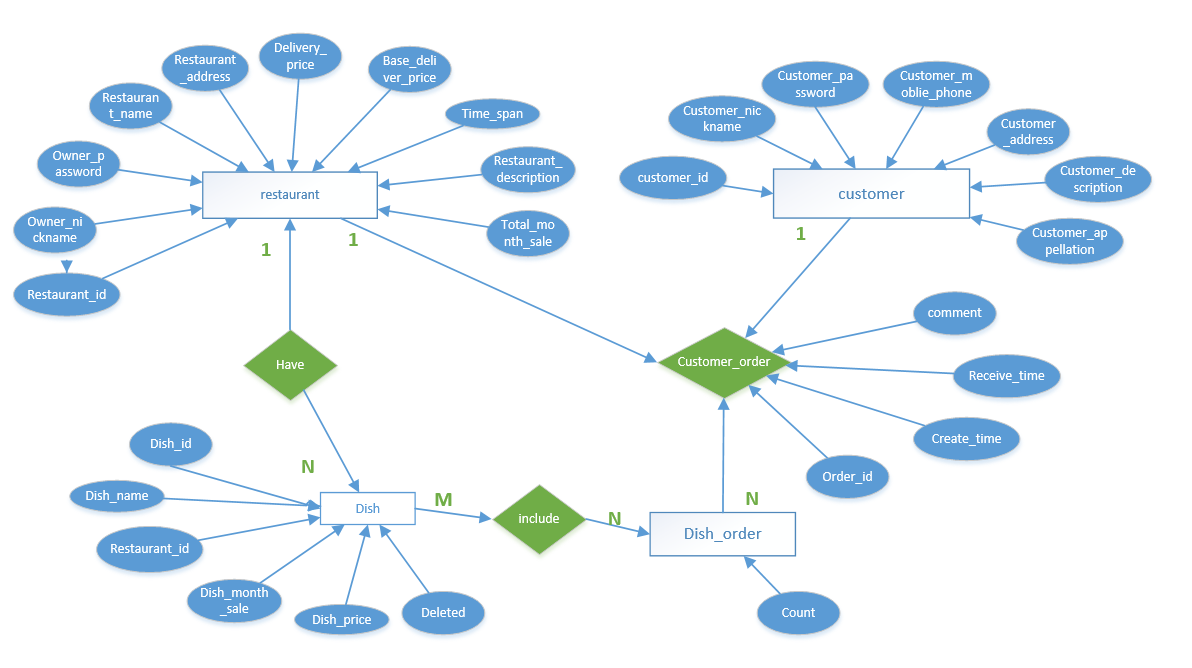
\includegraphics[width=5.00in,height=3.00in]{ER.png}
     \caption{\small{数据库ER图}}\label{fig:dummy}
  \end{figure}
 
 \item 关系图
  \begin{figure}[H]
    \centering
     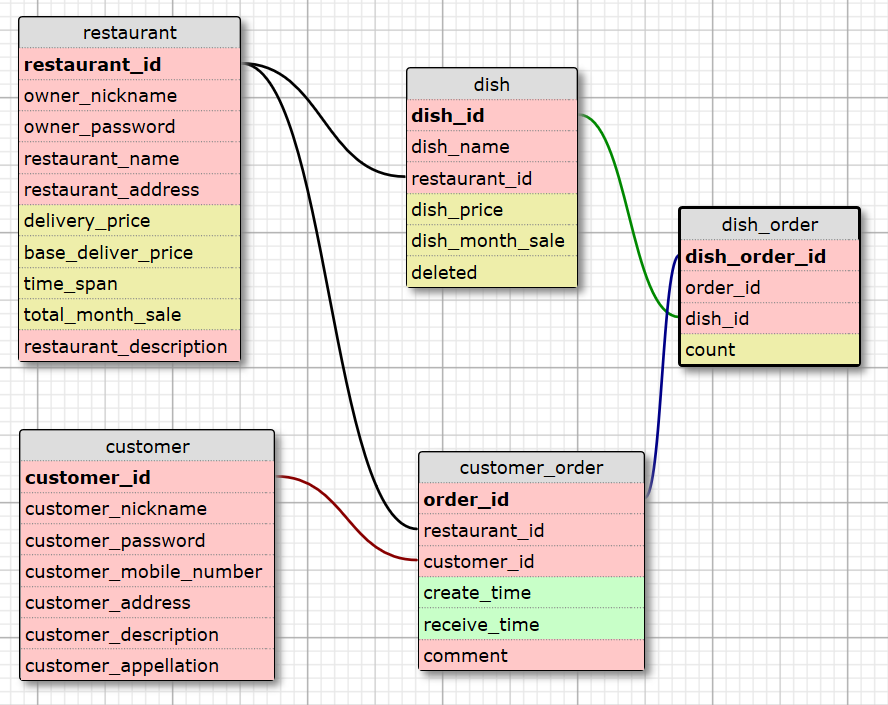
\includegraphics[width=6.00in,height=4.00in]{tables.png}
     \caption{\small{数据库表格关系图}}\label{fig:dummy}
  \end{figure}
  
 \item 建表语句
 \par\setlength{\parindent}{1em}\normalsize 数据库Glutton共包含5张表:商家表、用户表、菜品表、用户订单表、菜品订单表。
 \begin{itemize}
 \item \textbf{商家表}信息包括:商家号、用户名、密码、商家名、商家地址、配送费、起送价、平均配送时间、营业时间、月销量、商家公告,主键为商家号。
 \item \textbf{用户表}信息包括:用户号、用户名、密码、手机号、收获地址、用户个人信息、称呼,主键为用户号,其中用户手机号应该是唯一的,加UNIQUE区分。
 \item \textbf{菜品表}信息包括:菜品号、菜品名、所属商家号、菜品价格、菜品月销量,主键为菜品号,外键为所属商家号,即可将菜品与商家联系起来。其中,商家删除菜品后,不能影响用户历史订单对这个菜品显示,所以加deleted属性。当商家删除菜品后,deleted为true,该菜品不在商家中显示,而用户历史订单中仍然可以查询到。
 \item \textbf{用户订单表}信息包括:商家号、用户号、用户订单号、创建时间、收货时间、评论,主键为用户订单号,外键商家号、用户号分别关联商家表和用户表。
 \item \textbf{菜品订单表}信息包括:菜品订单号、用户订单号、菜品号、菜品数量,主键为菜品订单号,外键用户订单号、菜品号分别关联用户订单表和菜品表。这种设计使一个订单可以表示多个菜品,并减少了数据冗余。
 \end{itemize}
  \begin{figure}[H]
   \begin{minipage}[t]{0.5\linewidth}
    \centering
     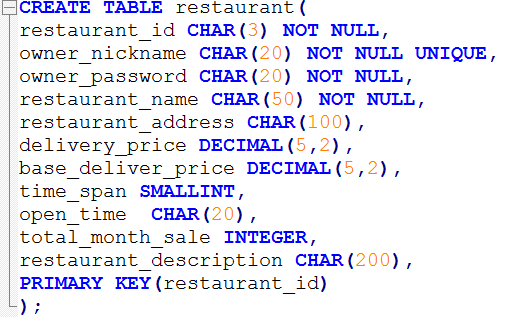
\includegraphics[width=3.2in]{table1.png}
     \caption{\small{创建商家表}}\label{fig:dummy}
   \end{minipage}
   \begin{minipage}[t]{0.5\linewidth}
    \centering
     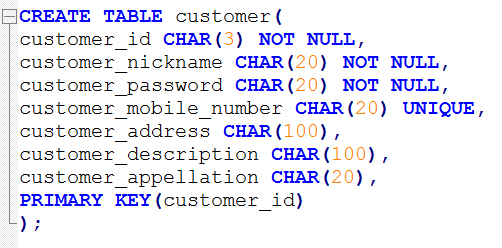
\includegraphics[width=3.2in]{table2.png}
      \caption{\small{创建用户表}}\label{fig:dummy}
   \end{minipage}
   \begin{minipage}[t]{0.5\linewidth}
    \centering
     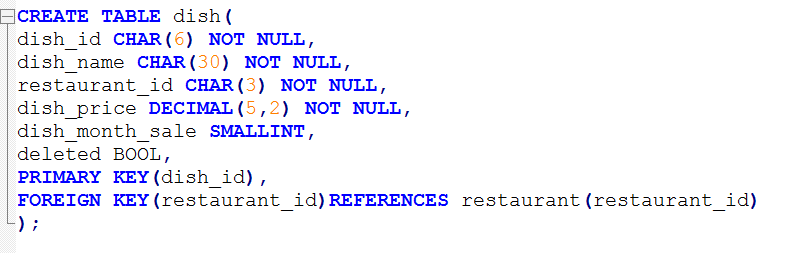
\includegraphics[width=3.2in]{table3.png}
     \caption{\small{创建菜品表}}\label{fig:dummy}
   \end{minipage}
   \begin{minipage}[t]{0.5\linewidth}
    \centering
     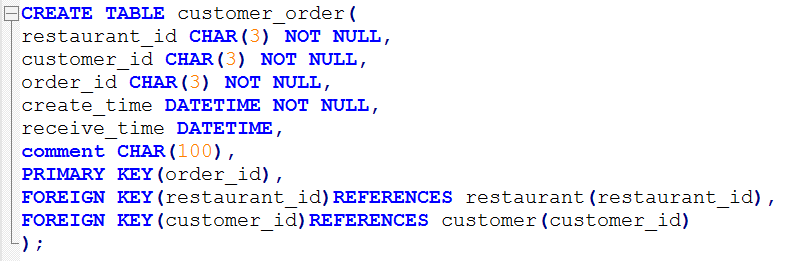
\includegraphics[width=3.2in]{table4.png}
     \caption{\small{创建用户订单表}}\label{fig:dummy}
   \end{minipage}
   \begin{minipage}[t]{0.5\linewidth}
    \centering
     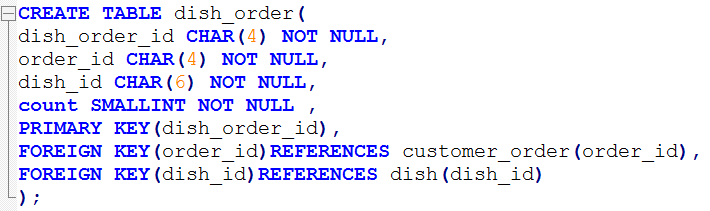
\includegraphics[width=3.2in]{table5.png}
     \caption{\small{创建菜品订单表}}\label{fig:dummy}
   \end{minipage}
  \end{figure}
  
 \item 插入语句
  \begin{description}
  利用INSERT语句向数据库中插入商家和菜品信息。示例如下:\\
  \item 商家信息:INSERT INTO restaurant VALUES('001','restaurant1','password','学城粥铺','上海市浦东新区张江镇华佗路572号',2,0,45,'09:00-23:00',743,' 需要米饭的亲们,可以在商品里面点哦,我们的炒菜是不配米饭的,除了商务套餐和盖浇饭以外,敬请谅解');\\
  \item 菜品信息:INSERT INTO dish VALUES('003-01','(大杯)红茶玛奇朵','003',15,717);
  \end{description}
  
 \item 查找语句-创建视图语句
 \item 更改语句
 \item 删除语句
 \end{itemize}


\end{document}
